\documentclass[aspectratio=169]{beamer}

\usepackage[utf8]{inputenc}
\usepackage[english]{babel}
\usepackage[T1]{fontenc}
\usepackage{lmodern}
\usepackage{bbm}
\usepackage{listings}
\usepackage{multicol}
\usepackage{csquotes}
\usepackage{hyperref}
\usepackage{indentfirst}
\usepackage{amsthm}
\usepackage{amsfonts}
\usepackage{amsmath}
\usepackage{amssymb}
\usepackage{mathtools}
\usepackage{tikz}
\usepackage{xcolor}
\usepackage{array}
\usepackage{bookmark}
\usepackage{booktabs}
\usepackage[inkscapeformat=png]{svg}

\newcommand{\id}[1]{\ensuremath{\mathit{#1}}}
\newcommand{\kw}[1]{\ensuremath{\mathtt{#1}}}
\newcommand{\Let}{\kw{let}}
\newcommand{\In}{\kw{in}}
\newcommand{\If}{\kw{if}}
\newcommand{\Then}{\kw{then}}
\newcommand{\Else}{\kw{else}}
\newcommand{\Filter}{\kw{filter}}
\newcommand{\Or}{\kw{or}}
\newcommand{\Groupby}{\kw{groupby}}
\newcommand{\Partition}{\kw{partition}}
\newcommand{\Scatter}{\kw{scatter}}
\newcommand{\Hist}{\kw{hist}}
\newcommand{\Map}{\kw{map}}
\newcommand{\Scan}{\kw{scan}}
\newcommand{\Sum}{\kw{sum}}
\newcommand{\Mod}{\kw{mod}}
\newcommand{\Fst}{\kw{fst}}
\newcommand{\Snd}{\kw{snd}}
\newcommand{\Presum}{\kw{presum}}
\newcommand{\True}{\kw{true}}
\newcommand{\False}{\kw{false}}
\newcommand{\Sort}{\kw{sort}}
\newcommand{\Segor}{\kw{segor}}
\newcommand{\Hash}{\kw{hash}}
\newcommand{\Random}{\kw{random}}
\newcommand{\Iota}{\kw{iota}}
\newcommand{\Unzip}{\kw{unzip}}
\newcommand{\Unit}{\mathbf{unit}}
\newcommand{\Int}{\mathbf{int}}
\newcommand{\Bool}{\mathbf{bool}}
\newcommand{\Def}{\kw{def}}
\newcommand{\While}{\kw{while}}
\newcommand{\Do}{\kw{do}}
\newcommand{\Rep}{\kw{rep}}
\newcommand{\Zip}{\kw{zip}}

\usetikzlibrary{automata, positioning, arrows}

\definecolor{mint}{HTML}{B8E6D9}
\definecolor{deepteal}{HTML}{1B7A6B}
\definecolor{fuseA}{HTML}{C1603F}
\definecolor{fuseB}{HTML}{0047AB}

\newcolumntype{M}[2]{>{\centering\arraybackslash}m{#1}<{\rule{0pt}{#2}}}
\newcommand{\darkmint}{mint!70!black}
\setbeamercolor{background canvas}{bg=mint}

\usetheme{default}
\usecolortheme{wolverine}
\setbeamercolor*{palette primary}{bg=deepteal, fg=white}
\setbeamercolor*{palette quaternary}{bg=deepteal, fg=white}
\setbeamercolor{structure}{fg=deepteal}
\setbeamertemplate{navigation symbols}{\insertframenumber/\inserttotalframenumber}
\setbeamertemplate{blocks}[rounded][shadow]
\setbeamercolor{block title}{bg=structure, fg=white}
\setbeamercolor{block body}{bg=structure!20!mint, fg=black}
\setbeamercolor{block title alerted}{bg=structure, fg=white}
\setbeamercolor{block body alerted}{bg=structure!20!mint, fg=black}
\setbeamercolor{block title example}{bg=structure, fg=white}
\setbeamercolor{block body example}{bg=structure!20!mint, fg=black}
\setbeamercolor{frametitle}{bg=deepteal, fg=white}

\setbeamertemplate{itemize item}{\scriptsize$\blacksquare$}
\setbeamertemplate{itemize subitem}{\scriptsize$\blacksquare$}
\setbeamertemplate{itemize subsubitem}{\scriptsize$\blacksquare$}

\title[optimisations for GPU]{What optimisations are worthwhile for filter, partition, and tokenisation on GPU?}
\author{\textbf{Lilje Henrich Due} \inst{1} \and Troels Henriksen \inst{1} \and Cosmin Eugen Oancea \inst{1}}
\institute[shortinst]{\inst{1} Department of Computer Science, University of Copenhagen}
\date{August 20th, 2026}


\begin{document}

\begin{frame}
  \begin{center}
    \titlepage
    \vfill
    \usebeamerfont{institute} Contact: \url{due@di.ku.dk}
  \end{center}
\end{frame}

\begin{frame}{Motivation}
  \begin{itemize}
    \item Primitive Operations
    \begin{itemize}
      \item Filter
      \item Partition
    \end{itemize}
    \item Non-uniform Data-Parallism
    \begin{itemize}
      \item Hash Maps
      \item Quick Sort
      \item Segmented Reduce
    \end{itemize}
    \item Pointer Structures
    \begin{itemize}
      \item Expression Evaluation
      \item Union-Find
      \item List Ranking
    \end{itemize}
  \end{itemize}
\end{frame}

\begin{frame}{Filter written in Futhark}
\vspace{1em}

\visible<2->{{\bfseries Example using an is even predicate:} {\ttfamily as = [0, 1, 2, 3, 4, 5]}.}
\vspace{10pt}

\vspace{0.5em}
\begin{tabular}{ll}
{\ttfamily\small\textbf{def} filter [n] 'a (p: a -> bool) (as: [n]a) : []a =} & \\[0.3em]
{\ttfamily\small\quad\textbf{let} flags = map p as} & \visible<3->{$[\id{t}, \id{f}, \id{t}, \id{f}, \id{t}, \id{f}]$}\\[0.3em]
{\ttfamily\small\quad\textbf{let} offsets = scan (+) 0 (map bool.i64 flags)} & \visible<4->{$[1, 1, 2, 2, 3, 3]$}\\[0.3em]
{\ttfamily\small\quad\textbf{let} is = map2 (\textbackslash f o -> if f then o - 1 else -1)} & \\
{\ttfamily\small\phantom{\quad\textbf{let} is = map2 (}flags} & \\
{\ttfamily\small\phantom{\quad\textbf{let} is = map2 (}offsets} & \visible<5->{$[0, {\scriptstyle -}1, 1, {\scriptstyle -}1, 2, {\scriptstyle -}1]$}\\[0.3em]
{\ttfamily\small\quad\textbf{let} result = scatter (copy as) is as} & \visible<6->{$[0, 2, 4, 3, 4, 5]$}\\[0.3em]
{\ttfamily\small\quad\:\:\textbf{in} take~offsets[n - 1]~result} & \visible<7->{$[0, 2, 4]$}\\[0.3em]
\end{tabular}
\vfill
{\tiny \textasteriskcentered{} copied array is actually a scratch array}
\end{frame}

\begin{frame}{Filter written in Futhark}
\vspace{1em}

{\ttfamily\small
\textbf{def} filter [n] 'a (p: a -> bool) (as: [n]a) : []a = \\[0.3em]
\quad\only<1->{\color{fuseA}}\textbf{let} flags = map p as \\[0.3em]
\quad\only<1->{\color{fuseA}}\textbf{let} offsets = scan (+) 0 (map bool.i64 flags) \\[0.3em]
\quad\only<1->{\color{fuseB}}\textbf{let} is = map2 (\textbackslash f o -> if f then o - 1 else -1) flags offsets \\[0.3em]
\quad\only<1->{\color{fuseB}}\textbf{let} result = scatter (copy as) is as} \\[0.3em]
\quad\:\:\textbf{in} take~offsets[n - 1]~result

\visible<2->{
\begin{center}
\resizebox{\textwidth}{!}{%
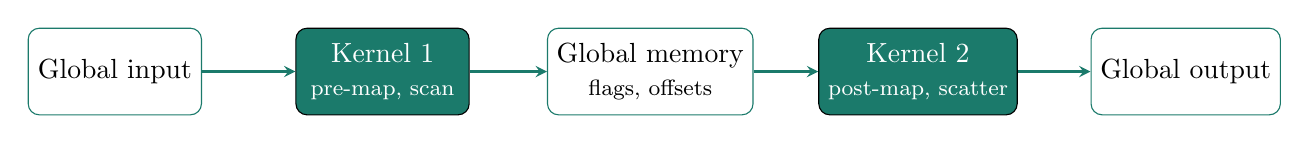
\begin{tikzpicture}[
  box/.style={draw, rounded corners, minimum width=2.2cm, minimum height=1.1cm, align=center, font=\normalsize},
  kernelbox/.style={box, fill=deepteal, text=white},
  memBox/.style={box, fill=white, draw=deepteal},
  arr/.style={->, >=stealth, thick, deepteal}
]

\node[memBox] (in1) at (-6.8,3) {Global input};
\node[kernelbox] (k1) at (-3.4,3) {Kernel 1 \\ \footnotesize pre-map, scan};
\node[memBox] (g1) at (0,3) {Global memory \\ \footnotesize flags, offsets};
\node[kernelbox] (k2) at (3.4,3) {Kernel 2 \\ \footnotesize post-map, scatter};
\node[memBox] (out1) at (6.8,3) {Global output};

\draw[arr] (in1) -- (k1);
\draw[arr] (k1) -- (g1);
\draw[arr] (g1) -- (k2);
\draw[arr] (k2) -- (out1);

\end{tikzpicture}%
}
\end{center}
}
\end{frame}

\begin{frame}{Filter written in CUDA}
\begin{center}
\resizebox{\textwidth}{!}{%
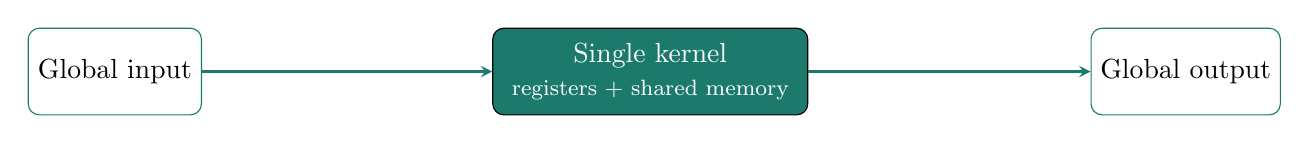
\begin{tikzpicture}[
  box/.style={draw, rounded corners, minimum width=2.2cm, minimum height=1.1cm, align=center, font=\normalsize},
  kernelbox/.style={box, fill=deepteal, text=white},
  memBox/.style={box, fill=white, draw=deepteal},
  arr/.style={->, >=stealth, thick, deepteal}
]

\node[memBox] (in2) at (-6.8,0) {Global input};
\node[kernelbox, minimum width=4cm] (k) at (0,0) {Single kernel \\ \footnotesize registers + shared memory};
\node[memBox] (out2) at (6.8,0) {Global output};

\draw[arr] (in2) -- (k);
\draw[arr] (k) -- (out2);

\end{tikzpicture}%
}
\end{center}

\begin{itemize}
  \item Streaming Scan.
  \item Avoid global memory round-trip.
  \item Not the only optimisation.
\end{itemize}
\end{frame}

\begin{frame}{Methodology}
\begin{itemize}
  \item Many hand-written CUDA kernels.
  \item Baseline is a two-kernel implementation mirroring compiler-generated code:
  \begin{itemize}
    \item Kernel 1: map + scan
    \item Kernel 2: map + scatter
  \end{itemize}
  \item Single-kernel implementations are compared against this baseline.
  \item Vary optimisations.
\end{itemize}
\end{frame}

\begin{frame}{Hand-Written CUDA Prototypes of Filter}
\begin{center}
  \small Relative speedup over \textbf{2K} baseline (higher is better) \\[0.5em]
  \small Datasets vary by \% of elements written: \textbf{Empty} (0\%) $\to$ \textbf{Full} (100\%) \\[1em]
\begin{tabular}{l|c|c|c|c|c}
  \textbf{Implementation} & \textbf{Full} & \textbf{Dense} & \textbf{Moderate} &
  \textbf{Sparse} & \textbf{Empty} \\
  \hline
  \textbf{2K} (baseline) & $1\times$ & $1\times$ & $1\times$ & $1\times$ & $1\times$ \\
  \textbf{1K} & $3.5\times$ & $3.7\times$ & $4\times$ & $4.4\times$ & $4.9\times$ \\
  \textbf{B} & $3.5\times$ & $3.7\times$ & $4.3\times$ & $4.9\times$ & $5.7\times$ \\
  \textbf{CW} & $3.4\times$ & $3.6\times$ & $3.8\times$ & $4.2\times$ & $5.7\times$ \\
  \textbf{FSMW} & $3.5\times$ & $3.8\times$ & $4.2\times$ & $5\times$ & $5.9\times$ \\
\end{tabular}
\end{center}
\vfill
\begin{center}
\tiny
\textbf{2K}: two-kernel baseline \quad
\textbf{1K}: single kernel \quad
\textbf{B}: bitsets in registers \quad
\textbf{CW}: coalesced writing to global memory \quad
\textbf{FSMW}: fewer shared memory writes
\end{center}
\end{frame}

\begin{frame}{Fusion of IR}
\begin{center}
\resizebox{\textwidth}{!}{%
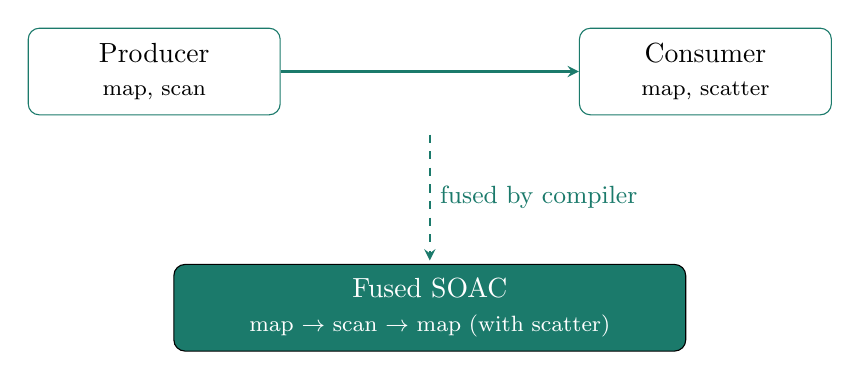
\begin{tikzpicture}[
  box/.style={draw, rounded corners, minimum width=3.2cm, minimum height=1.1cm, align=center, font=\normalsize},
  primbox/.style={box, fill=white, draw=deepteal},
  fusedbox/.style={box, fill=deepteal, text=white, minimum width=6.5cm},
  arr/.style={->, >=stealth, thick, deepteal}
]

% Before fusion: two separate producer/consumer screma
\node[primbox] (p) at (-3.5,3) {Producer \\ \footnotesize map, scan};
\node[primbox] (c) at (3.5,3) {Consumer \\ \footnotesize map, scatter};
\draw[arr] (p) -- (c);

\draw[arr, dashed] (0,2.2) -- node[right, font=\small] {fused by compiler} (0,0.6);

\node[fusedbox] (f) at (0,0) {Fused SOAC \\ \footnotesize map $\to$ scan $\to$ map (with scatter)};

\end{tikzpicture}%
}
\end{center}

\vspace{0.3cm}
\begin{center}
\small No source language fused primitive --- only \texttt{map}, \texttt{scan}, and \texttt{scatter}, combined by fusion.
\end{center}
\end{frame}

\begin{frame}{Scatter as IR}
\begin{align*}
  & \kw{scanscatter}~\id{f}~(\oplus)~\id{g}~\id{as}~\id{ds} = \\
  & \quad \Let~(\id{bs}, \id{gs})~=~(\Unzip\circ \Map~\id{f})~\id{as} \\
  & \quad \Let~\id{bs'}~=~\Scan~(\oplus)~\id{bs} \\
  & \quad \Let~(\id{is}, \id{vs}, \id{ss})~=~(\Unzip_3 \circ \Map_2~\id{g})~\id{bs'}~\id{gs} \\
  & \quad \Let~\id{ds'}~=~\Scatter~\id{ds}~\id{is}~\id{vs} \\
  & \quad \In~(\id{ds'}, \id{ss})
\end{align*}
\end{frame}

\begin{frame}{Accumulators}
\begin{itemize}
  \item Write-only array view; updates accumulate in place.
  \item Linear types.
  \item $[](\kw{acc}~\tau) \cong \kw{acc}~\tau$ --- so \Map~can take and return accumulators.
\end{itemize}

\begin{align*}
  \kw{with\_acc} &: []\tau \to (\kw{acc}~\tau \to \kw{acc}~\tau) \to []\tau \\
  \kw{update\_acc} &: \kw{acc}~\tau \to \Int \to \tau \to \kw{acc}~\tau
\end{align*}

\vspace{0.2cm}
Scatter, expressed via accumulators:
\begin{align*}
  \kw{with\_acc}~(\lambda \id{acc} \to \Map_2~(\lambda \id{i}~\id{v} \to \kw{update\_acc}~\id{acc}~\id{i}~\id{v})~\id{is}~\id{vs})~\id{ds}
\end{align*}
\end{frame}

\begin{frame}{Generalization of IR}
\begin{align*}
  & \kw{maposcanomap}~\id{f}~(\oplus)~\id{g}~\id{as} = \\
  & \quad \Let~(\id{bs}, \id{gs})~=~(\Unzip \circ \Map~\id{f})~\id{as} \\
  & \quad \Let~\id{bs'}~=~\Scan~(\oplus)~\id{bs} \\
  & \quad \In~\Map_2~\id{g}~\id{bs'}~\id{gs}
\end{align*}

\begin{gather*}
\visible<2->{
  \Scan~\oplus \equiv \kw{maposcanomap}~(\lambda a \to (\id{f} a, ()) )~(\oplus)~(\lambda a~\_ \to a)~\id{as} \\[20pt]
}
\visible<3->{
  \kw{scanomap}~\id{f}~\oplus \equiv \kw{maposcanomap}~\id{f}~(\oplus)~(\lambda a~b \to (a, b))~\id{as}
}
\end{gather*}

\end{frame}

\begin{frame}{Results: Filter}
\begin{center}
\begin{tabular}{l|c|c|c|c|c}
  \textbf{Method} & \textbf{Full} & \textbf{Dense} & \textbf{Moderate} &
  \textbf{Sparse} & \textbf{Empty} \\
  \hline
  \textbf{Old Futhark} & $1\times$ & $1\times$ & $1\times$ & $1\times$ & $1\times$ \\
  \textbf{New Futhark} & $3.5\times$ & $3.6\times$ & $4\times$ & $4.4\times$ & $4.5\times$
\end{tabular}

\vspace{20pt}

\visible<2->{
\begin{tabular}{l|c|c|c|c|c}
  \textbf{Method} & \textbf{Full} & \textbf{Dense} & \textbf{Moderate} &
  \textbf{Sparse} & \textbf{Empty} \\
  \hline
  \textbf{New Futhark} & $1\times$ & $1\times$ & $1\times$ & $1\times$ & $1\times$ \\
  \textbf{CUB} & $1\times$ & $1.1\times$ & $1.1\times$ & $1.2\times$ & $1.2\times$
\end{tabular}
}
\end{center}
\end{frame}

\begin{frame}{Results: Partition}
\begin{center}
\begin{tabular}{l|c|c|c|c|c}
  \textbf{Method} & \textbf{Full} & \textbf{Dense} & \textbf{Moderate} &
  \textbf{Sparse} & \textbf{Empty} \\
  \hline
  \textbf{Old Futhark} & $1 \times$ & $1\times$ & $1\times$ & $1\times$ & $1\times$ \\
  \textbf{New Futhark} & $2.5\times$ & $2.6\times$ & $2.6\times$ & $2.6\times$ & $2.3\times$
\end{tabular}

\vspace{20pt}

\visible<2->{
\begin{tabular}{l|c|c|c|c|c}
  \textbf{Method} & \textbf{Full} & \textbf{Dense} & \textbf{Moderate} &
  \textbf{Sparse} & \textbf{Empty} \\
  \hline
  \textbf{New Futhark} & $1\times$ & $1\times$ & $1\times$ & $1\times$ & $1\times$ \\
  \textbf{CUB} & $1.4\times$ & $1.4\times$ & $1.4\times$ & $1.4\times$ & $1.4\times$
\end{tabular}
}
\end{center}
\end{frame}

\begin{frame}{Results: Tokenizer}
\begin{center}
\begin{tabular}{l|c|c|c}
  \textbf{Method} & \textbf{Dense} & \textbf{Moderate} & \textbf{Sparse} \\
  \hline
  \textbf{Old Futhark} & $1\times$ & $1\times$ & $1\times$ \\
  \textbf{New Futhark} & $1.6\times$ & $1.8\times$ & $2\times$
\end{tabular}

\vspace{20pt}

\visible<2->{
\begin{tabular}{l|c|c|c}
  \textbf{Method} & \textbf{Dense} & \textbf{Moderate} & \textbf{Sparse} \\
  \hline
  \textbf{New Futhark} & $1\times$ & $1\times$ & $1\times$ \\
  \textbf{2K} & $1.8\times$ & $1.2\times$ & $1.1\times$
\end{tabular}
}
\end{center}

\begin{itemize}
  \item Simulates DFA.
  \item Determines location and token type.
\end{itemize}
\end{frame}

\begin{frame}{Conclusion}
\begin{itemize}
  \item Review of hand-written optimisations.
  \item A simple language extension that generalizes fusion.
  \item High-level programs become competitative to hand-written code.
\end{itemize}
\vspace{10pt}
\begin{columns}
  \begin{column}{0.5\textwidth}
    \begin{center}
      \textbf{Benchmarks} \\[0.5em]
      
\includegraphics[width=.6\linewidth]{images/benchmarks.png}
    \end{center}
  \end{column}
  \begin{column}{0.5\textwidth}
    \begin{center}
      \textbf{Futhark} \\[0.5em]
      
\includegraphics[width=.6\linewidth]{images/futhark.png}
    \end{center}
  \end{column}
\end{columns}
\end{frame}
\end{document}
\end{document}
